\cleardoublepage
\vspace*{\stretch{1}}
\begin{center}
  \begin{minipage}{\textwidth}
  \part*{Annexes}
\end{minipage}
\end{center}
\vspace*{\stretch{1}}

\newpage
\thispagestyle{empty}
\vspace*{\stretch{1}}
\begin{center}
  \begin{minipage}{\textwidth}
    \hrule
    \vspace{0.5cm}
    {\it  Cette partie, contenant les annexes de ce manuscrit, présente des
      travaux réalisés pendant la thèse mais pas assez aboutis ou trop
      éloignés du sujet de ce manuscrit pour y figurer à part
      entière. Cette partie se divise en deux sous-parties. La
      première correspond à l'annexe~\ref{ann:JFPC} et
      présente l'étude du cas discret du problème d'ordonnancement
      continu à contraintes énergétiques (article publié aux
      Journées Francophones de la Programmation par
      Contraintes~\cite{Nattaf_JFPC}). Ce paragraphe présente
      nottament un modèle de programmation par contraintes pour la
      restriction discrète du problème.

      La seconde annexe (ann.~\ref{ann:IESM}) porte sur la mise en place d'une
      matheuristique pour un problème industriel d'ordonnancement avec
      contraintes et objectifs énergétiques. Ce travail s'inscrit dans
      le cadre d'une collaboration pour le projet franco-chilien ECOS C13E04 et a
      été publié dans la conférence IESM (International Conference on
      Industrial Engineering and Systems
      Management~\cite{Nattaf_IESM}). Ce paragraphe présente tout
      d'abord le problème étudié, puis, dans un second temps, trois
      modèles de programmation linéaire à événements sont introduits. Les deux
      premiers, constituant des méthodes de résolution exacte,
      comportent un nombre de variables et de contraintes trop
      important pour expérer les résoudre en temps raisonnable. De ce
      fait, un troisième modèle simplifié est présenté et la solution
      de ce modèle est utilisée comme solution de base des modèles
      exacts.}   
    \vspace{0.5cm}
    \hrule
  \end{minipage}
\end{center}
\vspace*{\stretch{1}}

\chapter{Programmation linéaire mixte et programmation par contraintes
  pour un problème d'ordonnancement à contraintes énergétiques}  
\chaptermark{PLNE et PPC
  pour un problème à contraintes énergétiques}
\label{ann:JFPC}
Nous considérerons un problème d'ordonnancement cumulatif dans
lequel les tâches ont une durée et un profil de consommation de
ressource variable. Ce profil, qui peut varier en fonction du temps, est
une variable de décision du problème dont dépend la durée de la tâche
associée. 
Pour ce problème NP-difficle, nous présentons un modèle de programmation
par contraintes et un modèle de programmation linéaire en nombres
entiers (PLNE). De plus, des inégalités valides déduites de la
programmation par contraintes  viennent renforcer le PLNE. 
Ces modèles sont ensuite comparés par le biais d'expérimentations.


\section{Introduction}

Nous étudions un problème d’ordonnancement avec ressource continue et
contraintes énergétiques, le Continuous Energy-Constrained Scheduling
Problem (CECSP). Dans ce problème, un ensemble de tâches ${\cal
A}=\{1,\dots,n\}$ utilisant une ressource continue et cumulative de
capacité limitée $B$ doit être ordonnancé.  La quantité de ressource
nécessaire à l'exécution d'une tâche n'est pas fixée mais - le profil
de consommation de cette dernière est une fonction $b_i(t)$ définie
pour tout  $t \in \mathbb{R}$\footnote{Le domaine de définition de la
fonction peut être réduit mais, pour faciliter les notations, nous
supposons qu'elle est définie pour tout $t \in \mathbb{R}$.} - doit
être déterminé. Une fois la tâche commencée et jusqu'à sa date de fin,
la fonction $b_i(t)$ doit être comprise entre une valeur maximale,
$\bmax$, et minimale, $\bmin$.   

De plus, la consommation, à un instant $t$, d'une partie de
la ressource permet la production d'une certaine quantité d'énergie
et, une tâche finit lorqu'elle a reçu une énergie $W_i$. Cette
énergie est calculée par le biais d'une fonction de rendement $f_i$, 
propre à chaque tâche. Dans cet article, ces fonctions sont supposées
continues, croissantes, affines et peuvent être exprimées de la
manière suivante: 
 
\noindent
  $f_i(b)=\left\{
    \begin{array}{ll} 0 & \quad \text{si }b=0\\ a_i*b+c_i &\quad
                                                            \text{si }\bmin=0\text{ et }b \in ]\bmin,\bmax] \\ a_i*b+c_i &\quad
                                                                                                                           \text{si }\bmin\neq 0 \text{ et }b \in [\bmin,\bmax]
    \end{array} \right.$ 
  
  \noindent
  avec $a_i>0$ et $c_i \geq -a_i*\bmin $ pour
  s'assurer que $f_i(b) \geq 0,\ \forall b \in \inter[\bmin][\bmax]$.

Dans la suite, nous dénotons par $\ES$ et $\LS$
la date de début au plus tôt et au plus tard de $i$ et par
$\EE$ et $\LE$ la date de fin au plus tôt et au
plus tard de $i$.

Pour trouver une solution pour le CECSP, nous devons déterminer, pour
chaque tâche $i \in {\cal A}$, sa date de début $st_i$, sa date de fin
$et_i$ et sa fonction d'allocation de ressource $b_i(t)$, $\forall t
\in {\cal T}=[\min_{i\in{\cal A}} \ES, \max_{i\in {\cal
    A}} \LE]$. De plus, ces variables doivent satisfaire
les contraintes suivantes:
\begin{eqnarray} 
  \ES\le st_i < et_i \le \LE & & \forall i \in
{\cal A} \label {tw_CECSP}\\
  \bmin \le b_i(t) \le \bmax & & \forall i \in {\cal A},\
\forall t \in [st_i,et_i] \label {bminmax_CECSP}\\
  b_i(t)=0 & & \forall i \in {\cal A},\ \forall t \not\in
[st_i,et_i] \label {b0_CECSP}\\
  \int_{st_i}^{et_i} f_i(b_i(t))dt =W_i & & \forall i \in {\cal
A} \label{nrj_CECSP}\\
  \sum_{i \in {\cal A}} b_i(t) \le B & & \forall t \in {\cal
T} \label{res_CECSP}
\end{eqnarray}
L'objectif auquel nous nous sommes intéressés est la minimisation de
la consommation totale de la ressource. Dans~\cite{Nattaf2015}, les
auteurs montrent que trouver une solution admissible pour le CECSP est
déjà un problème NP-complet. 

De plus, une instance ayant des données seulement entières peut
n'avoir que des solutions à valeurs dans
$\mathbb{R}$~\cite{Nattaf2015}. Cependant, une dilatation de
l'instance, i.e. multiplier les données par un certain coefficient
$\alpha$, permet de palier à ce problème. 
De ce fait et dans le but de résoudre des instances entières, nous
nous sommes intéressés, dans un premier temps, à la version discrète
du CECSP, le DECSP (Discrete Energy Constrained Scheduling
Problem). Dans ce problème, toutes les données sont supposées entières
et les domaines de chaque variable ne contiennent
que des valeurs entières, i.e. $st_i,\ et_i,\ b_i(t) \in \mathbb{N}$ et
$b_i(t)$ est défini $\forall t \in {\cal T}_{\cal D}=\{\min_{i\in{\cal
A}} \ES,\dots, \max_{i\in {\cal A}} \LE\}$. 

Pour ce problème, nous présentons un modèle de
programmation par contraintes (PPC) permettant l'utilisation des
algorithmes de propagation mis en place pour la contrainte
cumulative, notamment~\cite{Gay2015}.  Un modèle de
programmation linéaire en nombres entiers (PLNE) est aussi
présenté. Ce modèle est ensuite renforcé à l'aide d'inégalités
valides déduites du raisonnement énergétique~\cite{Lopez1990}. 
Ces deux modèles sont ensuite testés sur des instances à données
entières, avec et sans dilatation.

\section{Modèle de programmation par contraintes}

Pour modéliser le DECSP à l'aide de la PPC, nous divisons chaque tâche
$i$ en deux sous-tâches $i_{min}$ et $i_{preem}$. La première,
$i_{min}$, est une tâche ayant une consommation de ressource fixe,
égale à $\bmin$, et une durée variable $p_i$. Cette tâche
représente la quantité de ressource obligatoirement consommée par une
activité durant son exécution, i.e. $\bmin$.  La seconde, $i_{preem}$
est une tâche préemptive optionnelle, consommant une quantité variable
de ressource comprise entre $0$ et $\bmax-\bmin$ et devant s'exécuter
en même temps que $i_{min}$. Cette tâche est elle-même divisée en
sous-tâches $i_{preem}^\ell,\ \ell \in \{1,\dots, et_i-st_i\}={\cal L}_i$. Notons
que $|{\cal L}_i|=et_i - st_i \le \lceil \frac{W_i}{f_i(\bmin)}\rceil$. 
\begin{ex}
Considérons la tâche possédant les attributs suivant:  $\ES= 0$,
$\LE=6$, $W_i=28$, $r^{min}=1$,
$r^{max}=5$ et $f_i(b)=2b+1$. La Figure~\ref{fig:ex:PPC} présente un
ordonnancement de cette tâche (à droite) et l'ordonnancement
correspondant donné par le modèle (à gauche) avec $r_{i^2_{preem}}=0$. 
\begin{figure}[!htb]
  \centering
  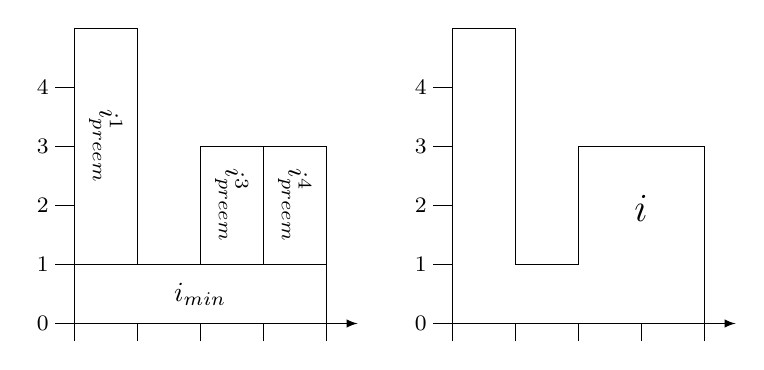
\begin{tikzpicture}
[xscale=0.8,yscale=0.75]
\node (O) at (0,0) {};
\draw (0,0) rectangle (4,1) node[midway] {$i_{min}$};
\draw (0,1) rectangle (1,5) node[midway,rotate=-90] {$i_{preem}^1$};
\draw (2,1) rectangle (3,3) node[midway,rotate=-90] {$i_{preem}^3$};
\draw (3,1) rectangle (4,3) node[midway,rotate=-90] {$i_{preem}^4$};

\draw[->,>=latex] (0,0) -- (4.5,0);

\foreach \i in {0,...,4}
{
  \draw (\i,-0.3) -- (\i,0);
  \draw (-0.3,\i) -- (0,\i)node[left=0.2cm] {\footnotesize \i};
}

\draw (7,5) -- (7,1) -- (8,1) -- (8,3)  -- node[below=0.5cm,midway] {\Large $i$}(10,3)  --  (10,1)
-- (10,0)--  (6,0) -- (6,5) -- cycle;
\draw[->,>=latex] (6,0) -- (10.5,0);

\foreach \i in {0,...,4}
{
  \draw (\i+6,-0.3) -- (\i+6,0);
  \draw (5.7,\i) -- (6,\i) node[left=0.2cm] {\footnotesize \i}; 
}    
  \end{tikzpicture}
  \caption{Exemple de solution du modèle PPC.}
  \label{fig:ex:PPC}
\end{figure}
\end{ex}
Le problème du DECSP peut alors être formulé à l'aide des variables:
\begin{itemize}
\item $i_{min}=\{s_{i_{min}}, e_{i_{min}}, b_{i_{min}},p_{i_{min}}\},\ 
  \forall i \in {\cal A}$ 
\item $i_{preem}^\ell=\{s_{i_{preem}^\ell},e_{i_{preem}^\ell},
  b_{i_{preem}^\ell},p_{i_{preem}^\ell}\}$, $\forall i \in {\cal A},\
  \ell \in {\cal L}_i$.
\end{itemize}
et des contraintes:
\begin{enumerate}  
\item $\forall (i,l) \in {\cal A} \times {\cal L}_i:\
  e_{i_{preem}^\ell} = s_{i_{preem}^{\ell+1}}$ 
\vspace{0.2cm}
\item $\forall i \in {\cal A}:\  s_{i_{min}} = s_{i_{preem}^1}$ et $ e_{i_{preem}^{|{\cal L}_i|}} = e_{i_{min}}$   
\vspace{0.2cm}
\item $\forall t \in  {\cal T}:\\ \sum\limits_{\substack{i \in {\cal A} \\ t \in [s_{i_{min}},e_{i_{min}}[}} b_{i_{min}}
  + \sum\limits_{\substack{(i,l) \in {\cal A}\times {\cal L}_i\\ t \in
      [s_{i_{preem}^\ell},e_{i_{preem}^\ell}[}}
  b_{i_{preem}^\ell} \le B$ 
\vspace{0.2cm}
\item $\forall i \in {\cal A}:\ \sum_{l \in {\cal L}_i} \left(f_i(b_{i_{preem}^\ell})
    (e_{i_{preem}^\ell}-s_{i_{preem}^\ell})\right) +
  f_i(b_{i_{min}}) (e_{i_{min}}-s_{i_{min}}) \ge W_i $
\end{enumerate}
La première contrainte permet d'ordonner les sous-tâches de
$i_{preem}$. Ceci dans le but de faciliter la modélisation des autres
contraintes. La seconde contrainte modélise le fait que $i_{preem}$
commence et finit en même temps que $i_{min}$. La troisième contrainte
assure que la capacité de la ressource n'est pas excédée en sommant, à
un instant $t$, les consommations minimales des tâches en cours ainsi
que les consommations des sous-tâches préemptives en cours. Enfin, la
quatrième contrainte permet de s'assurer que chaque tâche reçoit au
moins l'énergie requise $W_i$. 

Un des avantages de cette formulation est qu'elle permet l'utilisation
des algorithmes de propagation mis en places pour la contrainte
cumulative tels que le time-table classique~\cite{Baptiste2001},
disjonctif~\cite{Gay2015} ou associé au edge-finding~\cite{Vilim2011},
le raisonnement disjonctif~\cite{Baptiste2001}, ou encore le
raisonnement énergétique~\cite{Lopez1990}. Cependant, certains de ces
raisonnements peuvent être adaptés pour 
prendre en compte l'ensemble du problème. C'est le cas, par exemple,
du raisonnement énergétique détaillé ci-dessous.

\subsection{Raisonnement énergétique}


Ce paragraphe présente un algorithme de propagation pour le
DECSP basé sur le raisonnement énergétique défini pour le
CECSP~\cite{Nattaf2015}.  L'adaptation de ce raisonnement au cas
discret est quasi-directe. Cependant, nous rappelons les bases de
celui-ci car nous l'utiliserons dans la suite pour déduire des
inégalités valides pour le PLNE.

Le principe du raisonnement énergétique est de comparer la quantité de
ressource disponible dans un intervalle avec la quantité minimale de
ressource consommée par toutes les tâches dans cet intervalle.

Les configurations pour lesquelles la quantité de ressource requise
par une tâche $i$ dans l'intervalle $[t_1,t_2[$ est minimale
correspondent toujours à une configuration où la tâche reçoit le
maximum d'énergie possible, i.e. est ordonnancée à $\bmax$, en dehors
de $[t_1,t_2[$, tout en respectant les contraintes
\eqref{tw_CECSP}--\eqref{res_CECSP}. Ceci correspond donc à une des
configurations suivantes:
\begin{itemize}
\item la tâche est calée à gauche: ordonnancée à $\bmax$ durant
$[ \ES , t_1 [$;
\item la tâche est calée à droite: ordonnancée à $\bmax$ durant
$[t_2,\LE{[}$;
\item la tâche est centrée: ordonnancée à $\bmax$ durant
$[\ES,t_1[ \cup [t_2,\LE{[}$ ou ordonnancée à
$\bmin$ durant $[t_1,t_2[$.
\end{itemize} En effet, dans le dernier cas, il peut arriver
qu'ordonnancer la tâche à $\bmax$ dans $[\ES,t_1[ \cup
[t_2,\LE{[}$ implique que la quantité d'énergie restant à
apporter à la tâche dans $[t_1,t_2[$ ne soit pas suffisante pour
ordonnancer la tâche à $\bmin$ durant $[t_1,t_2[$. Or, ceci
impliquerait une violation de la
contrainte~\eqref{bminmax_CECSP}. Dans ce cas, la tâche est donc
ordonnancée à $\bmin$ durant l'intervalle $[t_1,t_2[$. Alors la
quantité de ressource requise par la tâche $i$ dans $[t_1,t_2[$ est la
quantité minimale requise par ces configurations.  

Les intervalles $[t_1,t_2[$ sur lesquels appliquer ce test pour le
CECSP sont décrits dans~\cite{Nattaf2015}. Pour le DECSP, nous devons
considérer les projections de ces intervalles sur les entiers,
i.e. $[a,b[ \rightarrow [\lfloor a \rfloor, \lceil b \rceil[$.  Les
ajustements pour le CECSP s'adaptent aussi naturellement au DECSP à
l'aide de cette même projection.

\section{Modèle de programmation linéaire en nombres entiers}
\label{MIP}
\subsection{Modèle}
La formulation proposée dans cet article est une formulation indexée par
le temps. Elle est adaptée de la formulation décrite
dans~\cite{Nattaf2015}. 
Dans ces formulations, l'horizon de temps est divisé en
intervalles de taille 1 et est défini par: ${\cal T}_{\cal D}$. 
Pour chaque activité $i \in {\cal A}$ et pour chaque instant $t \in
{\cal T}_{\cal D}$, nous définissons deux variables binaires $x_{it}$
et $y_{it}$ pour modéliser le début et la fin des activités. La
variable $x_{it}$ (resp. $y_{it}$) prendra la valeur $1$ si et
seulement si l'activité $i$ commence (finit) à l'instant $t$.
Pour modéliser la consommation de ressource et l'apport en énergie,
nous introduisons deux variables, $b_{it}$ et $w_{it}$ qui
représentent respectivement la quantité de
ressource consommée par l'activité $i$ dans la période de temps
$t$ et l'énergie reçue par cette même activité durant cette période. 

Par manque de place, ce modèle n'est pas entièrement décrit ici mais
nous décrivons les contraintes permettant de lier les variables
$b_{it}$ et $w_{it}$, i.e. permettant de calculer l'énergie apportée à
$i$ dans la période $t$, $w_{it}$ , en fonction de la consommation de
ressource $b_{it}$. Nous donnons aussi le nombre de variables et de
contraintes du modèle.

Les contraintes liant $b_{it}$ et $w_{it}$, $\quad \forall t\in {\cal T}_{\cal D},\
\forall i \in {\cal A}$ sont les suivantes:
\begin{equation}  w_{it}=a_ib_{it}+c_i\left(\sum_{\tau=\ES}^t
x_{i\tau}-\sum_{\tau=\ES+1}^t y_{i\tau}\right)  \label{conv_CECSP_TI}
\end{equation} Cette contrainte nous permet de modéliser la fonction
de rendement $f_i,\ \forall i \in {\cal A}$. En effet,
$\left(\sum_{\tau=\ES}^t x_{i\tau}\right.$ $\left.-\sum_{\tau=\ES+1}^t
y_{i\tau}\right) $ est égale à $1$ si et seulement si l'activité $i$
est en cours à l'instant $t$.  Dans ce cas là, la valeur de l'énergie
apportée à $i$ est bien $w_{it}=a_ib_{it}+c_i$. Le second cas se
produit quand l'activité $i$ n'est pas en cours à $t$. Dans ce cas,
$b_{it}=0$ implique $w_{it}=0$.

Le modèle possède donc $2n|{\cal T}_{\cal D}|$ variables binaires,
$2n|{\cal T}_{\cal D}|$ variables continues et au plus $3n+|{\cal
T}_{\cal D}|*(6n+1)$ contraintes.

\section{Inégalités valides basées sur le raisonnement énergétique}
Ce paragraphe décrit des inégalités valides déduites du raisonnement
énergétique pour le PLNE. Soit ${\cal R}$ l'ensemble des intervalles
d'intérêt pour le raisonnement énergétique.
\begin{align}
&(x_{i\ES} + y_{i\LE} -1 ) \, \bb + \sum_{j\neq i}
  \bb[j] \le \nonumber\\ 
&  B(t_2-t_1) \quad \forall i \in {\cal A},\ \forall
  [t_1,t_2] \in {\cal R}
\label{both}\\[2mm] 
&(x_{i\ES} + \sum_{t=t_1}^{t_2}y_{it} -1) \, \bb + \sum_{j\neq i}
  \bb[j] \le \nonumber \\
&  B(t_2-t_1) \quad \forall i \in {\cal A},\ \forall
  [t_1,t_2] \in {\cal R}
\label{left}\\[2mm] 
&(\sum_{t=t_1}^{t_2}x_{it} + y_{i\LE}-1) \, \bb + \sum_{j\neq i}
  \bb[j] \le \nonumber\\
&  B(t_2-t_1) \quad \forall i \in {\cal A},\ \forall
  [t_1,t_2] \in {\cal R}
\label{right}\\[2mm] 
&(1-\sum_{t<t_1}x_{it} - \sum_{t>t_2}y_{it}) \, \bb + \sum_{j\neq i}
  \bb[j] \le \nonumber \\
&  B(t_2-t_1) \quad \forall i \in {\cal A},\ \forall
  [t_1,t_2] \in {\cal R}
\label{total}\\[2mm] 
&(\sum_{t\le t_1}x_{it} + \sum_{t\ge t_2}y_{it} -1 ) \, \bb  \le
B(t_2-t_1) \nonumber\\
&\forall i \in {\cal A},\ \forall
[t_1,t_2] \in {\cal R}
\label{min}
\end{align}

L'inégalité~\eqref{both} correspond au cas où la tâche est centrée et est
ordonnancée à $\bmax$ durant $[\ES,t_1] \cup
[t_2,\LE{]}$. En effet, cette inégalité n'est active que dans
le cas où $(x_{i\ES} + y_{i\LE} -1 )= 1 \Rightarrow
\left[x_{i\ES}=1\land y_{i\LE}=1\right]$. Or,
ceci implique que la tâche commence à $\ES$ et finit
$\LE$. Donc, la ressource disponible dans $[t_1,t_2[$ doit
être suffisante pour donner la quantité de ressource minimale requise
par $i$ dans $[t_1,t_2[$ dans cette configuration.  Dans tous les
autres cas, l'inégalité devient $\sum_{j\neq i} \bb[j] \le B(t_2-t_1)$
ou $\sum_{j\neq i} \bb[j] - \bb \le B(t_2-t_1)$.

Les inégalités \eqref{left}, \eqref{right}, \eqref{total}, \eqref{min}
correspondent respectivement au cas où $i$ est calée à gauche, $i$ est
calée à droite, $i$ est complètement incluse dans $[t_1,t_2]$, $i$ est
exécutée à $\bmin$ durant l'intervalle $[t_1,t_2]$ et sont déduites de
la même façon que~\eqref{both}.  Ces inégalités seront ajoutées au
modèle indexé par le temps décrit à la section~\ref{MIP} pour
renforcer ce dernier. 
 
\section{Résultats expérimentaux}

Nous avons testé les différentes méthodes de résolution proposées dans
cet article sur les instances de~\cite{Nattaf2015}. Les
expérimentations ont été conduites sous le système d'exploitation
Ubuntu 64-bit 12.04 et les résultats sont calculés au moyen d'un
processeur 4-core, 8 thread Core (TM) i7-4770 CPU et de 8GB de mémoire
RAM. 

Le modèle de PLNE est résolu à l'aide de IBM Cplex 12.6 avec 2 threads
et une limite de temps de 100 secondes. Les inégalités déduites du
raisonnement énergétique sont calculées avant la résolution du PLNE et
ajoutées statiquement au modèle. Ceci augmente la taille du modèle de
$5|{\cal R}|n$ contraintes (avec $|{\cal R}| \in O(n^2)$). 

Le tableau~\ref{table1} décrit les résultats du PLNE. 

L'ajout des inégalités du raisonnement énergétique permet de résoudre
les instances à $25$ tâches de manières plus efficace. Cependant, elles
ralentissent le modèle pour les instances à $20$ ou $30$ tâches mais
la perte de rapidité dans ce cas là est beaucoup moins élevée que le
gain fait sur les instances à $25$. Une poursuite de recherche
intéressante serait d'essayer d'ajouter ces contraintes pendant la
résolution du PLNE en tant que coupes. 

Le modèle de PPC est résolu avec IBM CP Optimizer 12.6. Le
tableau~\ref{table2} décrit les résultats du modèle de PPC.  Le modèle 
de PPC est testé sans ajout du raisonnement énergétique présentés dans
cet article mais le modèle utilise les propagateurs du solveur. Des
résultats expérimentaux plus détaillées seront proposés lors de la
conférence.
\begin{table}
\centering
    \begin{tabular}{|c|c|cc|cc|}
      \hline
       & & \multicolumn{2}{c|}{$1^{ère}$ sol.} & \multicolumn{2}{c|}{fin algo.}\\
      \hline
    &  \#tâches & temps(s) &  écart & temps  & \%opt. \\
      \hline
      DEF	&	20	&	5.37	&	7.85	&	75.4	&	0.25\\
      ER	&	20	&	8.4	&	10.6	&	78.9	&	0.22\\
      \hline
      DEF	&	25	&	4.6	&	4.4	&	83.8	&	0.17\\
      ER	&	25	&	0.06	&	3.86	&	60.1	&	0.4\\
      \hline
      DEF	&	30	&	0.99	&	7.18	&	75.19	&	0.25\\
      ER	&	30	&	5.66	&	7.53	&	75.8	&	0.25\\
      \hline
    \end{tabular}
  \caption{Résultats du PLNE avec et sans inégalités valides: ER et
    DEF resp. (TL 1000s)}
  \label{table1}
\end{table}


\begin{table}
\centering
    \begin{tabular}{|c|cc|cc|}
      \hline
      & \multicolumn{2}{c|}{$1^{ère}$ sol.} & \multicolumn{2}{c|}{fin algo.}\\
      \hline
      \#tasks & time & deviation & time lim. &  \%solved \\
      \hline
20	&0.19&	34.1&	100&	95\\
25	&0.3	&47.9&	100	&91\\
30	&0.42	&43.1	&100	&95\\
      \hline
    \end{tabular}
  \caption{Résultats du modèle PPC}
\label{table2}
\end{table}

Les résultats montrent l'intérêt des inégalités valides ajoutées au
PLNE. Le modèle de PPC ne permet pas de prouver l'optimalité des solutions
trouvées mais a des résultats similaires au PLNE. En effet, dans
presque tous les cas, le modèle de PPC trouve une solution aussi bonne
que le PLNE, sans toutefois prouver son optimalité.

Les méthodes présentées ont aussi été testées sur des instances
dilatées dans le but de garantir l'existence de solutions entières.  
La dilatation est effectuée de la manière suivante. Soit $\alpha$ le
plus petit commun 
multiple à tous les $\bmin$ et $\bmax$. Alors, la dilatation
consiste à multiplier $\LE,\ \EE,\
\LS,\ \ES$ et $W_i$ par $\alpha$. Ces
expérimentations n'ont pas donné de résultats dû à la grande taille
de ces modèles. Les modèles continus pourraient donc rester  la
seule alternative pour obtenir des solutions optimales dans le cas où
la solution est réelle.

Parmi les poursuites de recherche possibles, on trouve l'amélioration
des modèles avec la réduction du nombre de variable et/ou de contraintes et la
mise en place d'algorithmes de propagation dédiés.
\section*{Bibliographie\markboth{}{BIBLIOGRAPHIE}}
\begin{bibunit}[alpha]
\nocite{JFPC}
\nocite*
\putbib[JFPC]
\end{bibunit}








\chapter{A batch sizing and scheduling problem on parallel machines with
different speeds, maintenance operations, setup times and energy
costs}
\chaptermark{Papier IESM}
\label{ann:IESM}

This paper considers a production scheduling problem in a Chilean
company from the metalworking industry. This company produces steel
balls of different diameters on parallel production lines. There are
different types of production lines and each production line may have a
different speed for producing each diameter. Furthermore a setup time
occurs when changing the diameter produced on each machine. Besides
these production and setup operations, maintenance operations have to
be scheduled. These electrical machines yield high energy
demands. It is therefore crucial to minimize total energy consumption,
which depends on batch/machine assignment, and maximum demand on peak
hours. We consider the batch sizing and scheduling problem involving
electricity costs in a non-uniform parallel machine context. Given a
demand for each family of steel balls, the problem consists in
splitting the demand in sublots (batches) that have to be assigned and
scheduled on the parallel machines together with the required
maintenance operations. The goal is to complete the schedule before a
common deadline while minimizing electricity costs. We propose to
tackle this problem through mixed integer linear programming. We
propose a global formulation and a two-phase
matheuristic. Computational results on realistic instances are
provided.

\section{Introduction}

This paper considers a production scheduling problem in a Chilean
company from the metalworking industry. The problem and the industrial
context was described in \cite{Urrutia:Thesis:2014}. This company
produces steel balls on parallel production lines. The steel balls are
obtained by roll forming or forging from a raw material consisting of
metal bars. The steel balls are mainly used in the copper and gold
mining industry for mineral grinding, i.e. for reducing the size of
the mineral particles to a maximal granularity that permits to remove
the major part of impurities from the mineral. There are several types
of steel balls to produce, each corresponding to a different ball
diameter. There are two types of production lines : roll formers for
small diameters and forges for larger diameters (although medium
diameter balls can be produced by both production line types). Each
production line may have a different speed for producing each
diameter. Furthermore a setup time occurs when changing the diameter
produced on each machine. Besides these production and setup
operations, maintenance operations have to be scheduled. These
machines are electrical and the production process results in high
energy demands. As mentioned in \cite{Urrutia:Thesis:2014}, up to 50\%
of the production cost in such a manufacturing process can be due to
electricity consumption. In Chile, as in many other places, different
electricity rates are applied for peak hours and off-peak hours. So it
can be crucial for metalworking companies to control the electricity
demand during peak hours. Planning the maintenance and setup
operations during the peak hours can be intuitively a policy that
favors electricity cost decrease.

In this paper we consider a batch sizing and scheduling problem
involving electricity costs in a non-uniform parallel machine
context. Given a demand for each family of steel balls, the problem
consists in splitting the demand in sublots (batches) that have to be
assigned and scheduled on the parallel machines together with the
required maintenance operations. The goal is to complete the schedule
before a common deadline while minimizing electricity costs. We
propose to tackle this problem through a mixed integer linear
programming approach.

Section \ref{sec:prob} presents the batch sizing and scheduling
problem. Section \ref{sec:review} is devoted to a brief presentation
of the related work. Section \ref{sec:milp} gives the proposed
mixed-integer linear programming (MILP) formulation. Section
\ref{sec:simple} gives a simplified MILP formulation that ignores the
peak costs and that serves as a basis for a matheuristic. Section
\ref{sec:exp} presents the considered realistic problem instances and
the results obtained by our approach. Section \ref{sec:concl} draws
concluding remarks and directions for future work.

\section{The industrial scheduling problem}
\label{sec:prob}

The problem involves a set ${\cal J}$ of $n$ lots (jobs) to be
scheduled on a set ${\cal M}$ of $m$ machines. There is total a
production demand $D_j$ for each job $j\in{\cal J}$ to be fulfilled
during the scheduling horizon given by a time interval $[0,T]$. Each
job $j\in{\cal J}$ can be split into a maximum number of $\lfloor
D_j/\epsilon \rfloor$ sublots (batches), where $\epsilon$ is the
minimum batch size. The machines able to produce a job $j$ are
gathered in set ${\cal M}_j$. For a given job $j\in{\cal J}$, a
machine $k\in {\cal M}_j$ has a production speed $v_{j}^{k}$. Whenever
a batch of a job $j\in{\cal J}$ is scheduled immediately after a batch
of job $i\in{\cal J}$ on a machine $k\in{\cal M}$, a setup time
$s_{ij}^k\geq 0$ is necessary on the machine. Each machine is assumed
to have a constant electrical power demand $w_k$. There are $H$ peak
periods within the horizon, each being defined by an interval
$[a_h,f_h)$ with $a_h<f_{h}$ for $h=1,\ldots,H$ and $f_h<a_{h+1}$ for 
  $h=1,\ldots,H-1$. Concerning cost minimization, we considered a
  weighted sum problem where $\alpha$ denotes the weight of the total
  energy consumption while $\beta$ denotes the weight of the maximum
  consumption during peak hours.

A solution consists in determining:
\begin{itemize}
\item A set of batches ${\cal B}_j$ with $|{\cal B}_j|=B_j\geq 1$, for
  each job $j\in{\cal J}$,
\item A production amount $q_{j,b}\geq \epsilon$, for each batch
  $b\in{\cal B}_j$,
\item The assignment $a_{j,b}$ of each batch $b \in {\cal B}_j$, i.e. 
  the line on which batch $b \in {\cal B}_j$ is produced,
\item A start time $S_{j,b}$, for each job $j\in{\cal J}$ and for each
  batch $b\in{\cal B}_j$.
\end{itemize}
Let ${\cal B}=\cup_{j\in{\cal J}}\{(j,b)|b\in{\cal B}_j\}$ denote the
set of pairs (job, batch index). Let ${\cal A}_k=\{(j,b)|a_{j,b}=k\}$ 
the set of batches assigned to machine $k\in{\cal M}$.

The problem constraints can be stated as follows:

%\noindent One and only one machine has to be assigned to each batch.
%\begin{eqnarray}{C}
%\left(\sum_{k\in{\cal M}}A_k=|{\cal B}|\right)\wedge
%\left(\mathop{\cup}_{k\in{\cal M}}{\cal A}_k={\cal
%  B}\right)\label{ct:1}
%\end{eqnarray}
A batch can only be assigned on an authorized machine.
\begin{eqnarray}
a_{j,b} \in {\cal M}_j \quad \forall j\in {\cal J},\forall b\in{\cal B}_j
\label{ct:2}
\end{eqnarray}

\noindent The demand must be satisfied for each job.
\begin{eqnarray}
\sum_{b\in{\cal B}_j} q_{j,b} = D_j\quad\forall j\in{\cal
  J}\label{ct:4}
\end{eqnarray}

\noindent The duration $p_{j,b}$ of a batch $b\in {\cal B}_j$ is equal to 
its production divided by the speed of its assigned machine.
\begin{eqnarray}
p_{j,b}=q_{j,b}/v_{j}^{a_{j,b}}\quad\forall
j\in{\cal J},\forall b\in{\cal B}_j\label{ct:5}
\end{eqnarray}


\noindent No batches assigned to the same machine may overlap and the
setup time between two consecutive batches on the same machine must be
respected.
\begin{eqnarray}{Cr}
S_{j,b}\geq S_{i,b'} + p_{i,b'}
+ s_{i,j}^{a_{j,b}} & \nonumber
\\ \forall (i,j) \in{\cal
  J}^2,\forall (b,b')\in{\cal B}_i\times{\cal B}_j \mbox{ such that } 
a_{i,b'}=a_{j,b}\label{ct:6}
\end{eqnarray}

\noindent All production must fit in the time horizon.
\begin{eqnarray}
S_{j,b}+p_{j,b}\leq T \quad \forall (j,b)\in{\cal B}\label{ct:7}
\end{eqnarray}

We need not introduce maintenance operations in the model. We consider
that there is a subset ${\cal J}^M$ of the jobs ${\cal J}$ that
correspond to maintenance operations. They concern a single machine
($|{\cal M}_j|=1$). The maintenance duration is given by $D_j$ and we
have $v^k_j=1$ for $k\in{\cal M}_j$. We denote by ${\cal B}^M$ the set
of batches corresponding to maintenance operations. We introduce last
the constraints that each maintenance job cannot be splitted:
\begin{eqnarray}
|{\cal B}_j|=1\quad\forall j\in{\cal J}^M\label{ct:8}
\end{eqnarray}
We assume that there is no required setup time between a maintenance
job and a production job. However me make the realistic assumption
that the maintenance duration is such that $D_j\geq s_{ii'}^k$, $\forall
j\in{\cal J}^M$, $\forall i,i'\in {\cal J}\setminus{\cal J}^M, i\neq
i', \forall k \in {\cal M}$, i.e. is larger than any other setup time. 
Furthermore we assume that all other setup times satisfy the triangle inequality
\begin{eqnarray}
s_{ij}^k\geq s_{il}^k+s_{lj}^k\quad\forall k\in{\cal M},\forall
i,j,l\in{\cal J}\setminus{\cal J}^M,i\neq j\neq l\nonumber
\end{eqnarray}

A solution is feasible if and only if it satisfies constraints
\ref{ct:2}--\ref{ct:8}.


There are two components linked to energy consumption. As the machines
have different speeds and different power consumptions, the first part
of the objective is to minimize the total electricity consumption $C$.
\begin{eqnarray}
C=\sum_{k\in{\cal M}} w_k\sum_{(j,b)\in{\cal A}_k\setminus{\cal
    B}^M}p_{j,b}\label{eq:obj2}
\end{eqnarray}
We are also interested in the maximum demand over the peak
periods. Let us define for convenience the set of batches in process
at a given time point $t$
\begin{eqnarray}
{\cal B}(t)=\{(j,b)\in{\cal B}|S_j,b\leq t <
S_{j,b}+p_{j,b}\}\label{eq:obj4}
\end{eqnarray}
Then the maximum demand over peak hours is equal to
\begin{eqnarray}
P_{\max}=\max_{h\in{\cal H}}\max_{t\in[a_h,b_h)}\sum_{k\in{\cal
      M},\exists(j,b)\in{\cal B}(t)\cap{\cal A}_k\setminus{\cal
      B}^M}w_k\label{eq:obj5}
\end{eqnarray}
Remark that maintenance operations are excluded in the computation of
these costs.  Then the problem objective can be written
\begin{eqnarray}
\min \alpha C + \beta P_{\max}\label{eq:obj}
\end{eqnarray}


Note that the problem is NP-hard as the problem of finding a solution
has the decision variant of the parallel machine problem as special
case.  The above-defined constraints can be used to check the
feasibility and cost of a solution in polynomial time but they cannot
be implemented as is in a mathematical programming solver.

We present a small example and its optimal solution. Consider $n=3$
jobs on $m=2$ lines with demands $D_1=10$, $D_2=12$, $D_3=6$. There is
one peak period $h=1$ with $a_h=2$ and $b_h=4$ and a common deadline
of $T=6$ for all jobs and maintenance operations. There are two
maintenance operations ${\cal J}^M=\{4,5\}$ of duration $D_4=2$ on
machine $1$ and $D_5=1$ on machine $2$ to be performed also before the
deadline. Machine power demands are $w_1=w_2=10$.  For each job,
authorized machines are ${\cal M}_1=\{1,2\}$, ${\cal M}_2=\{1\}$,
${\cal M}_3=\{2\}$, ${\cal M}_3=\{2\}$, ${\cal M}_4=\{1\}$, ${\cal
  M}_5=\{2\}$.  Setup and speed matrices are respectively equal to
$$(s_{i,j}^1)_{i,j\in{\cal J}}=(s_{i,j}^2)_{i,j\in{\cal
    J}}=\left[\begin{array}{ccc}0&2&1\\1 & 0 &
    1\\1&1&0\end{array}\right]$$
$$(v_j^k)_{j\in{\cal J},k\in{\cal
    M}}=\left[\begin{array}{cc}2&3\\6&0\\0&2\end{array}\right]$$
Figure \ref{fig_smallex} presents an optimal solution for this example
where ${\cal B}_1=\{1,2\}$ (job $1$ is split into two batches), ${\cal
  B}_2={\cal B}_3=1$ (jobs $2$ and $3$ are scheduled in one batch).
Batch machine assignments are given by $a_{1,1}=M_1,\ a_{1,2}=M_2,\
a_{2,1}=M_1$ and $a_{3,1}=M_2$. Productions
inside each batch are given by $q_{1,1}=4$, $q_{1,2}=6$, $q_{2,1}=12$,
$q_{3,1}=6$. According to the assigned machine speeds, the batch
duration are given by $p_{1,1}=q_{1,1}/v_1^1=2$,
$p_{1,2}=q_{1,2}/v_1^2=2$, $p_{2,1}=q_{2,1}/v_2^1=2$,
$p_{3,1}=q_{3,1}/v_3^2=3$. The start times of the different batches
and of the maintenance operations (in gray) are displayed in the Gantt
chart. According to the machine power demand, total consumption of
machine 1 is $4\times w_1=40$ and total consumption of machine 2 is
$5\times 10=50$. Hence we obtain a total energy consumption of 90 and
a maximal demand on peak hours of 10. We observe that batch splitting
has been necessary to meet the deadline and minimize energy
consumption, while maintenance has been used to avoid large demands
during peak hours.
\begin{figure}[htbp]
\centering 
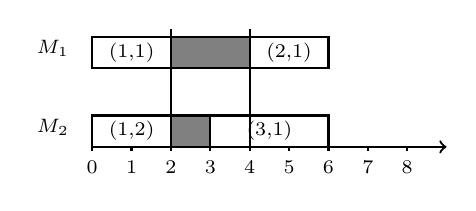
\begin{tikzpicture}[scale=0.50]
    \begin{scope}[thick,font=\scriptsize]
\draw[->] (0,0) -- coordinate (x axis mid) (9,0);
    	\foreach \x in {0,...,8}
     		\draw (\x,1pt) -- (\x,-3pt)
			node[anchor=north] {\x};

\node at (-1,0.5) {$M_2$};
\draw (0,0) rectangle (2,0.8) node [pos=0.5] {(1,2)};
\draw[fill=gray] (2,0) rectangle (3,0.8);
\draw (3,0) rectangle (6,0.8) node [pos=0.5] {(3,1)};

\node at (-1,2.5) {$M_1$};
\draw (0,2) rectangle (2,2.8) node [pos=0.5] {(1,1)};
\draw[fill=gray] (2,2) rectangle (4,2.8);
\draw (4,2) rectangle (6,2.8) node [pos=0.5] {(2,1)};

%\draw (2,0) rectangle (3,0.8) node [pos=0.5] {2};
%\draw[fill=gray] (3,0) rectangle (5,0.8);
%\draw (5,0) rectangle (6,0.8) node [pos=0.5] {3} ;
%\draw[fill=gray] (6,0) rectangle (7,0.8);
%\draw (7,0) rectangle (8,0.8) node [pos=0.5] {1};

\draw (2,0) -- (2,3);
\draw (4,0) -- (4,3);
%\node at (1.5,0.4) {$J_1$};
%\node at (4,0.4) {$J_2$};
\end{scope}
 \end{tikzpicture}  
\caption{Optimal solution of a simple instance}
\label{fig_smallex}
\end{figure}


Hence, after a brief presentation of the related work, we will
introduce a mixed-linear integer programming formulation.


\section{Related work and modeling issues}
\label{sec:review}

A vast literature considers upper level lot-sizing and scheduling
problems in parallel machine environment with setup times (such as in
\cite{james2011single,xiao2013mip}) involving, among others, inventory
costs and also using discrete time mixed-integer linear programming
formulations. First, the discrete time models do not fit our problem
as the duration of the sublot is a function of the sublot size (a
continuous variable) and the machine speed for the family of balls
corresponding to the sublot. Furthermore we do not have holding costs
in our model. More generally, our problem is in fact related to the
(operational) production scheduling level where it is assumed that
lots of products aiming at satisfying the demand in a given period
have already been constituted at the (tactical) planning level.

Lot streaming (also called lot splitting) is a known technique to
improve the performance of production scheduling environment at the
operational level \cite{dauzere1997lot,chang2005comprehensive} by
allowing to split the jobs across the different production stages or
lines.  In our case, the lot streaming process in simplified by the
fact that we have a single stage. This is also the reason why we
rather use the ``batch sizing'' term rather than lot streaming or
splitting (we borrowed this term from \cite{Hazir2014}).

The possibility of splitting the jobs (lots/batches) adds another
dimension to the decisions besides assignment of the jobs to the
machine and sequencing/scheduling of the job operations. Many lot
streaming/batch sizing and scheduling problems have been considered in
the literature for different scheduling context, including parallel
machine scheduling for which efficient algorithms are available
\cite{serafini1996scheduling,xing2000parallel}. However, these first
studies did not consider the presence of setup times that can be
needed on a machine between two sublots. This feature, that occurs in
our case when the ball diameter is changed, puts obviously a limit to
the interest of systematic job splitting.  Several approaches can be
found for parallel machine lot streaming/batch sizing problems with
setup times
\cite{Yalaoui2003,tahar2006linear,beraldi2008rolling}. Compared to
these previous works, our study is concerned with electricity cost
minimization objectives. In manufacturing, energy constraints and
costs are becoming crucial. Consequently, energy-related objectives
have been recently considered both in lot-sizing problems
\cite{absi2013lot} and in production scheduling problems
\cite{mouzon2007operational,artigues2013energy,german2015}. However to
our knowledge, reducing the energy consumption cost by an integrated
management of lot streaming/batch sizing, setup and maintenance
scheduling in a parallel machine scheduling environment is a novel
approach.

In this paper, one of the objective is to come up with a mixed-integer
linear programming formulation (MILP) of the problem. In scheduling
problems, there are standardly three categories of MILP formulations
\cite{queyranne1994}: the continuous time formulations with sequencing
variables, the continuous time formulations with positional (or
event-based) variables and the discrete time formulations. In the
considered problem, the continuous lot splitting possibility and the
variable machine speed combined with large time horizons would render
a discrete time formulation (such as the ones generally used in the
lot-sizing literature) impractical. Therefore we need a continuous
time formulation. Now looking at the conceptual continuous time
formulation (\ref{ct:2}--\ref{eq:obj}), most non-linear constraints
could be linearized in a standard way yielding a continuous time (also
called disjunctive) formulation with sequencing variables
$x_{j,b,i,b'}\in\{0,1\}$ where $x_{j,b,i,b'}=1$ if and only if batch
$(i,b')$ is scheduled after batch $(j,b)$ on the same machine. In
\cite{neron2001}, the authors consider such a formulation for a simple
identical parallel machine scheduling problem with job-splitting and
sequence-dependent setup times with the makespan criterion. In this
simple case splitting a job is only useful if all sublots are
scheduled on different machines, hence the authors consider binary
sequencing variables of the type $x_{i,j,k}$ where $x_{i,j,k}=1$ is
the sublot of job $i$ in machine $k$ is sequenced before the sublot of
job $j$ in machine $k$.  However in our case, it can be necessary to
have two batches of the same job on the same machine, especially due
to the interest of avoiding production during the peak hours. Among
many other configurations Fig.~\ref{fig_contrex-1batch} shows an
optimal solution for a $1$ machine and $3$ jobs example ($m=1$ and
$n=3$) with setup times $s_{12}=s_{21}=s_{13}=s_{31}=1$,
$s_{23}=s_{32}=2$, unit machine speed, unit machine power, demands
$D_1=2$, $D_2=D_3=1$, deadline $T=8$ and weights $\alpha=0$,
$\beta=1$. Setup times are shown in gray.  The optimal solution (of
cost $0$) needs to split job 1 in two batches to have no production
within the peak hour (interval marked with a P).


\begin{figure}[htbp]
\centering 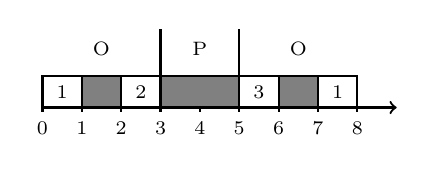
\begin{tikzpicture}[scale=0.50]
    \begin{scope}[thick,font=\scriptsize]
\draw[->] (0,0) -- coordinate (x axis mid) (9,0);
    	\foreach \x in {0,...,8}
     		\draw (\x,1pt) -- (\x,-3pt)
			node[anchor=north] {\x};
\draw (0,0) rectangle (1,0.8) node [pos=0.5] {1};
\draw[fill=gray] (1,0) rectangle (2,0.8);
\draw (2,0) rectangle (3,0.8) node [pos=0.5] {2};
\draw[fill=gray] (3,0) rectangle (5,0.8);
\draw (5,0) rectangle (6,0.8) node [pos=0.5] {3} ;
\draw[fill=gray] (6,0) rectangle (7,0.8);
\draw (7,0) rectangle (8,0.8) node [pos=0.5] {1};
\node at (1.5,1.5) {O};
\node at (4,1.5) {P};
\node at (6.5,1.5) {O};

\draw (3,0) -- (3,2);
\draw (5,0) -- (5,2);
%\node at (1.5,0.4) {$J_1$};
%\node at (4,0.4) {$J_2$};
\end{scope}
 \end{tikzpicture}  
\caption{Two batches of a job on the same machine}
\label{fig_contrex-1batch}
\end{figure}


Another issue for modeling the problem in continuous time is the
linearization of the expressions (\ref{eq:obj4}, \ref{eq:obj5})
defining the maximum demand over the continuous horizon. An important
remark is that the electricity consumption only changes at a batch
start or end time.  This clearly brings us to consider an event-based
model. These models consider a finite number of events and use an
event-indexed continuous variable to associate a start time to each
event and a binary variable to assign a batch start or end
time. Consequently, we can also associate a continuous variable
representing the total electricity consumption at a given event, that
shall not change until the next event.  Note that event-based models
were previously used for lot streaming and scheduling in hybrid
flow-shops \cite{defersha2012mathematical} and are also widely used in
batch scheduling in the process industry \cite{floudas2005mixed}. They
were also more recently introduced in resource-constrained project
scheduling problems \cite{KALM10d} and in scheduling problems under
energy constraints \cite{nataff2015}.

\section{A continuous time event-based mixed-integer linear programming formulation}
\label{sec:milp}

The event-based model we propose for the problem, is based on the fact
that energy consumption can only change at the beginning or at the end
of each batch. Hence we fix for each job its maximum number of batches
$B_j$ and we consider a set ${\cal E}$ of $2\sum_{j=1}^nB_j$
events. Now the start-end event-based formulation of the problem
involves the following decision variables (variables with domain
$[0,1]$ are continuous variables that will be set binary by the
constraints involving other binary variables).

\begin{itemize}
\item $t_e\geq 0$ is the time of event $e\in{\cal E}$.
\item $x_{j,b}^e\in\{0,1\}$ is equal to $1$ iff batch $(j,b)\in{\cal
  B}$ starts at event $e\in{\cal E}$.
\item $y_{j,b}^e\in\{0,1\}$ is equal to $1$ iff batch $(j,b)\in{\cal
  B}$ ends at event $e\in{\cal E}$.
\item $a_{j,b}^k\in\{0,1\}$ is equal to $1$ iff batch $(j,b)\in{\cal
  B}$ is assigned to machine $k\in{\cal M}$.
\item $x_{j,b}^{e,k}\in[0,1]$ auxiliary variable equal to product
  $x_{j,b}^ea_{j,b}^k$.
\item $y_{j,b}^{e,k}\in[0,1]$ auxiliary variable equal to product
  $y_{j,b}^ea_{j,b}^k$.
\item $o_{e,k}\in[0,1]$ is equal to $1$ iff machine $k\in{\cal M}$ is
  on at event $e\in{\cal E}$.
\item $p_{j,b}\geq 0$ is the production of batch $(j,b)\in{\cal B}$.
\item $P_{e,h}\in\{0,1\}$ models the relative positioning of
  intervals $[t_e,t_{e+1})$ and peak hour interval $[a_h,f_h)$ in the
      sense that $P_{e,h}=0\Rightarrow t_e\geq f_h$.
\item $P_{h,e}\in\{0,1\}$ models the relative positioning of
  intervals $[t_e,t_{e+1})$ and peak hour interval $[a_h,f_h)$ in the
      sense that $P_{h,e}=0\Rightarrow t_{e+1}\leq a_h$.
\item $P_e^k\in[0,1]$ models the fact that event $e$ is active on a peak hour on machine
  $k$ (i.e. $[t_e,t_{e+1})$ has a non-empty intersection with a peak
  hour interval and machine $k$ is on at event $e$).
\item $W_{j,b}\geq 0$ total electrical consumption of batch $(j,b)$.
\end{itemize}

The constraints can be expressed as follows. $M$ denotes a
sufficiently large integer.
\begin{eqnarray}
t_e\leq t_{e+1}\quad\forall e\in{\cal E}\setminus\{|{\cal
  E}|\}\label{ct:see:1}
\end{eqnarray}
Each batch $(j,b)$ has to be scheduled at most once.
\begin{eqnarray}
\sum_{e\in{\cal E}}x_{j,b}^e\leq1 \quad \forall (j,b)\in{\cal B}
\end{eqnarray}
\begin{eqnarray}
\sum_{e\in{\cal E}}y_{j,b}^e\leq 1 \quad \forall (j,b)\in{\cal B}
\end{eqnarray}
A started batch must be ended, and reciprocally.
\begin{eqnarray}
\sum_{e\in{\cal E}}y_{j,b}^e=\sum_{e\in{\cal E}}x_{j,b}^e \quad
\forall (j,b)\in{\cal B}
\end{eqnarray}
The end event of a batch cannot be lower than its start event.
\begin{eqnarray}
\sum_{f\in{\cal E},f\geq e}x^f_{j,b}\geq \sum_{f\in{\cal E},f\geq
  e}y^f_{j,b}\quad \forall (j,b)\in{\cal B}, \forall e\in{\cal E}
\end{eqnarray}
A batch has to be assigned to a machine to have a non-zero production
(as $B_j$ is the maximum number of batch for job $j$, there can be
some unassigned batches).
\begin{eqnarray}
p_{j,b}\leq\sum_{k\in{\cal M}_j}a_{j,b}^kD_j\quad \forall
(j,b)\in{\cal B}
\end{eqnarray}
A batch assigned to a machine must have a minimum size.
\begin{eqnarray}
p_{j,b}\geq\sum_{k\in{\cal M}_j}a_{j,b}^k\epsilon\quad \forall
(j,b)\in{\cal B}
\end{eqnarray}

A batch has to be assigned to at most one machine among the candidate
machines.
\begin{eqnarray}
\sum_{k\in{\cal M}_j}a_{j,b}^k\leq 1\quad \forall (j,b)\in{\cal B}
\end{eqnarray}
The following constraints are set on auxiliary variables
$x_{j,b}^{e,k}$ and $y_{j,b}^{e,k}$ to linearize products
$x_{i,b}^ea_{j,b}^k$ and $y_{i,b}^ea_{j,b}^k$.
\begin{eqnarray}
x_{j,b}^{e,k}\geq x_{j,b}^e+a_{j,b}^k-1\quad\forall (j,b)\in{\cal
  B},\forall e\in{\cal E},\forall k\in{\cal M}
\end{eqnarray}
\begin{eqnarray}
x_{j,b}^{e,k}\leq x_{j,b}^e\quad\forall (j,b)\in{\cal B},\forall
e\in{\cal E},\forall k\in{\cal M}
\end{eqnarray}
\begin{eqnarray}
x_{j,b}^{e,k}\leq a_{j,b}^k\quad\forall (j,b)\in{\cal B},\forall
e\in{\cal E},\forall k\in{\cal M}
\end{eqnarray}
\begin{eqnarray}
y_{j,b}^{e,k}\geq y_{j,b}^e+a_{j,b}^k-1\quad\forall (j,b)\in{\cal
  B},\forall e\in{\cal E},\forall k\in{\cal M}
\end{eqnarray}
\begin{eqnarray}
y_{j,b}^{e,k}\leq x_{j,b}^e\quad\forall (j,b)\in{\cal B},\forall
e\in{\cal E},\forall k\in{\cal M}
\end{eqnarray}
\begin{eqnarray}
y_{j,b}^{e,k}\leq a_{j,b}^k\quad\forall (j,b)\in{\cal B},\forall
e\in{\cal E},\forall k\in{\cal M}
\end{eqnarray}
A machine is on at an event $e$ depending on its status at the
preceding event and/or start or completion of a task on this machine
(we define also $o_{0,k}=\sum_{(j,b) \in {\cal B}}x_{j,b}^{0,k}$,
$\forall k\in{\cal M}$).
\begin{eqnarray}{Cr}
o_{e,k}=o_{e-1,k}-\sum_{(j,b)\in{\cal B}} y_{j,b}^{e,k} \nonumber\\ +
\sum_{(j,b)\in{\cal B}} x_{j,b}^{e,k}&\forall e\in{\cal E},\forall
k\in{\cal M}
\end{eqnarray}
%A machine can only run one batch at a time.
%\begin{eqnarray}
%o_{e,k}\leq 1\quad \forall e\in{\cal E},\forall k\in{\cal M}
%\end{eqnarray}
The common deadline must be satisfied.
\begin{eqnarray}
t_{|{\cal E}|}\leq T\label{eq25}
\end{eqnarray}
Setup times must be satisfied between two consecutive batches.
\begin{eqnarray}
t_f\geq t_e + s_{ij}^k ( x_{j,b}^{f,k}+y_{i,b'}^{e,k}-1 ) \quad
\forall e,f\in{\cal E}, f\geq e,\nonumber\\ \quad \quad \quad
\quad\forall (j,b),(i,b')\in{\cal B},(j,b)\neq(i;b'), \forall
k\in{\cal M}
\end{eqnarray}
Batches can be assigned only on authorized machines.
\begin{eqnarray}
a_{j,b}^k=0\quad\forall(j,b)\in{\cal B},\forall k\in{\cal
  M}\setminus{\cal M}_j
\end{eqnarray}
End and start time events of a batch have to be spaced according to
the batch duration on the assigned machine.
\begin{eqnarray}
t_f\geq t_e+p_{j,b}/v_{j,k}-M
(2-x_{j,b}^{e,k}-y_{j,b}^{f,k})\nonumber\\ \quad \quad \quad
\quad\forall e,f\in{\cal E}, f\geq e,\forall (j,b)\in{\cal B},\forall
k\in{\cal M}
\end{eqnarray}
\begin{eqnarray}
t_f\leq t_e+p_{j,b}/v_{j,k}+M
(2-x_{j,b}^{e,k}-y_{j,b}^{f,k})\nonumber\\ \quad \quad \quad
\quad\forall e,f\in{\cal E}, f\geq e,\forall (j,b)\in{\cal B},\forall
k\in{\cal M}
\end{eqnarray}
The demand of each job must be satisfied.
\begin{eqnarray}
\sum_{b\in{\cal B}_j} p_{j,b}=D_j\quad\forall j\in{\cal J}
\end{eqnarray}
The following constraints set the relative positioning of event $e$
and peak hour period $h$, in the sense that if $P_{e,h}=0$,
intersection of $[t_e,t_e+1)$ and peak hour interval $[a_h,f_h)$ is
    empty because $t_e\geq f_h$
\begin{eqnarray}
t_e\geq f_h(1-P_{e,h})\quad\forall e\in{\cal E},\forall h\in{\cal H}
\end{eqnarray}
The following constraints set the relative positioning of event $e$
and peak hour period $h$, in the sense that if $P_{h,e}=0$,
intersection of $[t_e,t_e+1)$ and peak hour interval $[a_h,f_h)$ is
    empty because $t_{e+1}\leq a_h$
\begin{eqnarray}
t_{e+1}-a_h \leq T P_{h,e}\quad\forall e\in{\cal E},\forall h\in{\cal
  H}
\end{eqnarray}



Machine $k$ is marked as active during peak hour at event $e$ whenever
machine $k$ is on at event $e$ and interval $[t_e,t_{e+1})$ intersects
  peak hour interval $[a_h,f_h)$.
\begin{eqnarray}
P_{e}^k\geq P_{e,h}+P_{h,e}+o_{e,k}-2\nonumber\\ \quad \quad \quad
\quad\quad \quad \quad \quad \forall e\in{\cal E},\forall h\in{\cal
  H},\forall k\in{\cal M}
\end{eqnarray}
The maximum demand objective is defined by the following constraints.
\begin{eqnarray}
P_{\max}\geq \sum_{k\in{\cal M}} w_kP_{e}^k\quad\forall e\in{\cal E}
\end{eqnarray}
The consumption of a batch depends on its duration and on the power of
its assigned machine.
\begin{eqnarray}
W_{j,b}\geq w_k p_{j,b} / v_{j,k} - M (1-a_{j,b}^k)\nonumber\\ \quad
\quad \quad \quad\quad \quad \quad \quad\forall (j,b)\in{\cal
  B}\setminus{\cal B}^M,\forall k\in{\cal M}
\end{eqnarray}

The objective function aims at minimizing the total consumption and
the maximum demand on peak hours.
\begin{eqnarray}
\min \alpha\sum_{(j,b)\in{\cal B}\setminus{\cal B}^M}W_{j,b} + \beta
P_{\max}\label{ct:objsee1}
\end{eqnarray}

The MILP model made of constraints (\ref{ct:see:1}-\ref{ct:objsee1})
is denoted as (MILP1). We now present an alternative model that
contains more binary variables but less constraints. Product variables
$x_{j,b}^{e,k}$ and $y_{j,b}^{e,k}$ can be considered as binary and
assignment variables $a^k_{j,b}$, as well as start and end variables
$x_{j,b}^e$ and $y_{j,b}^e$ can be eliminated by setting:
$$ a^k_{j,b}=\sum_{e\in{\cal E}}x_{j,b}^{e,k}\quad\forall(j,b)\in{\cal
  B},\forall k\in{\cal M}$$
$$ x_{j,b}^e=\sum_{k\in{\cal M}}x_{j,b}^{e,k}\quad\forall(j,b)\in{\cal
  B},\forall e\in{\cal E}$$
$$ y_{j,b}^e=\sum_{k\in{\cal M}}y_{j,b}^{e,k}\quad\forall(j,b)\in{\cal
  B},\forall e\in{\cal E}$$

The obtained model is denoted by (MILP2).

If we come back to Figure \ref{fig_smallex} example. We can use 5
global events with $t_1=0$, $t_2=2$, $t_3=3$, $t_4=4$ and $t_5=6$. For
MILP2, we have $x_{1,1}^{1,1}=y_{1,1}^{2,1}=1$,
$x_{1,2}^{1,2}=y_{1,2}^{2,2}=1$, $x_{2,1}^{4,1}=y_{2,1}^{5,1}=1$,
$x_{3,1}^{3,2}=y_{3,1}^{5,2}=1$ and for maintenance operations
$x_{4,1}^{2,1}=y_{4,1}^{4,1}=1$ and
$x_{5,1}^{3,2}=y_{5,1}^{5,2}=1$. For peak computation the only
concerned event is $e=3$ and we have $P_3^2=1$ because
$P_{3,1}+P_{1,3}+o_{3,2}=1$ (the event is inside the peak and the
machine is on).

\section{A simplified model and a matheuristic}
\label{sec:simple}

The models (MILP1) and (MILP2) proposed in Section \ref{sec:milp} have
several drawbacks. First they have a large number of binary variables
and constraints, especially constraints involving big-$M$ coefficient
that significantly weaken the LP relaxation. Second, finding a
solution that ends before the common deadline can be difficult and
even impossible in practice.

If we ignore the maximum consumption during peak hours, we can
simplify the model, transforming the event-based model into a
positional model.  We consider a set ${\cal E}_k$ of maximum
$\sum_{j=1}^nB_j$ positions on each machine $k$ and the following
reduced set of variables, including a tardiness variable for each job
aiming at relaxing the hard common deadline and including it into the
objective function.
\begin{itemize}
\item $t_{e,k}\geq 0$ is the start time of batch scheduled at position
  $e\in{\cal E}_k$ on machine $k\in{\cal M}$.
\item $x_{j,b}^{e,k}\in\{0,1\}$ is equal to $1$ if batch
  $(j,b)\in{\cal B}$ is assigned to position $e$ on machine $k$
\item $p_{j,b}^{e,k}\geq 0$ is the production of batch $(j,b)\in{\cal
  B}$ if it is scheduled at position $e$ on machine $k$.
\item $T_k\geq 0$ is the tardiness of machine $k\in{\cal M}$ in the
  case it finishes its production after the common deadline.
\end{itemize}
The problem constraints can then be expressed as follows.  The start
times of tasks at each position are ordered.
\begin{eqnarray}
t_{e,k}\leq t_{e+1,k}\quad\forall k\in{\cal M},\forall e\in{\cal
  E}_k\setminus\{|{\cal E}_k|\}\label{ct:simpl:1}
\end{eqnarray}
Each batch $(j,b)$ has to be scheduled at most once.
\begin{eqnarray}
\sum_{ k\in{\cal M}_j}\sum_{e\in{\cal E}_k}x_{j,b}^{e,k}\leq 1 \quad
\forall (j,b)\in{\cal B}
\end{eqnarray}
Each event on each machine $(e,k)$ corresponds to at most one batch.
\begin{eqnarray}
\sum_{(j,b)\in{\cal B}} x_{j,b}^{e,k}\leq 1 \quad \forall k\in{\cal
  M}_j,\ \forall e\in{\cal E}_k
\end{eqnarray}
The production of a batch $(j,b)$ at a position of a machine is 0 if
the batch is not assigned at this position on this machine.
\begin{eqnarray}
p_{j,b}^{e,k}\leq D_jx_{j,b}^{e,k}\quad \forall (j,b)\in{\cal
  B},\forall k\in{\cal M}_j, \forall e\in{\cal E}_k
\end{eqnarray}
A batch assigned to a position on a machine must have a minimum size
of $\epsilon$.
\begin{eqnarray}
p_{j,b}^{e,k}\geq \epsilon x_{j,b}^{e,k}\quad \forall (j,b)\in{\cal
  B},\forall k\in{\cal M}_j, \forall e\in{\cal E}_k
\end{eqnarray}
The demand of each job must be satisfied.
\begin{eqnarray}
\sum_{b\in{\cal B}_j} \sum_{ k\in{\cal M}_j}\sum_{e\in{\cal E}_k}
p^{e,k}_{j,b}=D_j\quad\forall j\in{\cal J}
\end{eqnarray}
Setup times must be satisfied between two consecutive batches.
\begin{eqnarray}
t_{e+1,k}\geq t_{e,k} + \sum_{(j,b)\in{\cal B}} p_{i,b}^{e,k} /
v_{i,k} + s_{ij}^k (
\sum_{b=1}^{B_i}x_{i,b}^{e,k}+\sum_{b'=1}^{B_j}x_{j,b'}^{e+1,k}-1 )
\nonumber\\\quad \forall e\in{\cal E}_k\setminus|{\cal E}_k|, \forall
i,j\in {\cal J}, i\neq j, \forall k\in{\cal M}
\end{eqnarray}
The following constraint computes the violation of the deadline
(tardiness) on machine k (in case a job is assigned to the last event,
its duration must be added).
\begin{eqnarray}
T_k\geq t_{|{\cal E}_k|} +\sum_{(j,b)\in{\cal B}}p_{j,b}^{e,k}- T
\quad \forall k\in{\cal M}
\end{eqnarray}

The objective function aims at minimizing a weighted sum of the total
tardiness and the total consumption.
\begin{eqnarray}
\min \gamma \sum_{k\in{\cal M}}T_k+\sum_{(j,b)\in{\cal B}} \sum_{
  k\in{\cal M}_j}\sum_{e\in{\cal E}_k} w_k p_{j,b}^{e,k} / v_{j,k}
\end{eqnarray}
where $\gamma$ is a coefficient large enough to ensure that the total
tardiness will be minimized in priority.

This model, denoted as (MILP3) is greatly simplified, however the
solution ignores peak hours.  Consequently in a second phase, The
solution of (MILP3) can serve as a basis of a matheuristic for further
improvement of the computed peak cost. To that purpose we compute a
global event set ${\cal E}'=\cup_{k\in{\cal M}}{\cal E}_k$ and we sort
the events according to their time $t_e$.  Then we can accelerate the
solution time of (MILP1) or (MILP2) by preassigning the start and end
times of activities to the event set according to the solution found
by (MILP3).

\section{Computational experiments}
\label{sec:exp}

The experiments are conducted on an Intel Core i7-4770 processor with
4 cores and 8 gigabytes of RAM under the 64-bit Ubuntu 12.04 operating
system. We use CPLEX 12.6 with 1 thread for solving the models. The
total time limit of 3050 seconds for solving both (MILP2) and (MILP3)
models: 3000 seconds for (MILP3) and 50 seconds for (MILP2).

The instances are extracted from the real instances of
\cite{Urrutia:Thesis:2014} and are as follows. For these instances,
the number of machines is equal to $3$, the time horizon is equal to
the number of hours in each month (e.g. in January, this number is
$31\times 24= 744$) and the machine consumption is constant and equal
to $10 MW$ for each machine.

Each instance has $10$ different lots and the setup time and the
speed of each machine are described by Table~\ref{table1} and
Table~\ref{table2} respectively. In Table~\ref{table2}, whenever the
speed of the machine is equal to zero then the lots can not be
scheduled on this machine.

\begin{table}[!htb]
  \begin{center}
    \normalsize
    \begin{tabular}{|c|cccccccccc|}
      \hline 
      \backslashbox{i}{j} & 1 & 2 & 3 & 4 & 5 & 6 & 7 & 8 & 9 &
      10\\ 
      \hline 
      1&0& 4& 5& 6& 7& 8& 1& 1& 0& 1\\
      2&4& 0 &4& 5& 6& 7& 1& 1& 0& 1\\ 
      3&5 &4 &0 &4 &5 &6 &1 &1 &1 &1 \\
      4&6 &5 &4 &0 &4 &5 &0 &2 &2 &2 \\
      5&7 &6 &5 &4 &0 &4 &1 &3 &3 &3 \\
      6&8 &7 &6 &5 &4 &0 &1 &4 &3 &4 \\
      7&4 &4 &5 &4 &4 &5 &0 &5 &2 &5 \\
      8&4 &4 &5 &6 &7 &8 &5 &0 &2 &5 \\
      9&4 &4 &5 &6 &7 &8 &5 &3 &0 &3 \\
      10&4 &4 &5& 6& 7& 8 &5 &5 &3 &0\\
      \hline
    \end{tabular}
    \vspace{0.1cm}
    \caption{setup times between batches}
    \label{table1}
  \end{center}
\end{table}

\begin{table}[!htb]
  \normalsize
  \begin{center}
    \begin{tabular}{|c|ccc|}
      \hline \backslashbox{lot}{line} & 1 & 2 & 3\\ \hline 1 & 0 & 4 &
      0\\ 2 & 0 & 5.1 & 0\\ 3 & 0 & 6 & 0\\ 4 & 8.1 & 8.9 & 0\\ 5 &
      9.5 & 9 & 0\\ 6 & 11 & 8.8 & 0\\ 7 & 10.6 & 0 & 4\\ 8 & 0 & 0 &
      5.4\\ 9 & 0 & 0 & 8.5\\ 10 & 0 & 0 & 8.1\\ \hline
    \end{tabular}
    \vspace{0.1cm}
    \caption{machine speeds for each lot}
    \label{table2}
  \end{center}
\end{table}

For each instance, the maintenance duration is equal to $120$ for each
machine. As in Chile, peak hours occurs from 6pm to 11pm, we set the
peak hours to these values in our instances.
\begin{table*}[t]
  \small
  \centering
  \begin{tabular}{|c|cccc|cccc|}
    \hline 
    & \multicolumn{4}{|c|}{MILP3}&
                                   \multicolumn{4}{|c|}{MILP2}\\ 
    \hline 
    \#batch & consump. & tard. & gap & time(s) &
                                                 peak & tard. & consump. & gap\\ 
    \hline
    \rule[-5pt]{0pt}{10pt}
    2	&	16711,54	&	19,39	&	49,56	&	25,2	&	30	&	18,41	&	16692,6	&	59,88	\\
    \rule[-5pt]{0pt}{10pt}
    3	&	16703,83	&	21,43	&	49,71	&	25,49	&	30	&	22,44	&	16699,8	&	71,21	\\
    \rule[-5pt]{0pt}{10pt}
    4	&	16743,19	&	27,41	&	56,8	&	29,22	&	30	&	26,85	&	16750,71	&	97,18	\\
    \hline
  \end{tabular}
  \caption{Results of experiments for (MILP2+MILP3)}
  \label{table4}
\end{table*}

Unfortunately, both model (MILP1) and (MILP2) can not be used alone to
find an optimal solution. Indeed, the great number of constraints and
variables prevent the solver from finding a solution, even a feasible
one. Therefore, in order to solve the problem, we use first 
(MILP3) and then, we use the solution to help (MILP2) to find a
feasible solution.

At the beginning of the procedure, i.e. before using (MILP3), we
use a simple heuristic to help the model finding a solution. This
heuristic considers only one batch for each different lot and schedule
this batch on the least loaded machine. This heuristic is described by
algorithm~\ref{algo1}. Maintenance operations are randomly set in such
a way that, on each machine, the end of the operation occurs before
the deadline, i.e. the end of the planning horizon $T$.

\begin{algorithm}[english]
  \caption{Simple heuristic for finding a simple solution}
\label{algo1}
  $machLoad_k=0,\ \forall k \in {\cal M}$ 
  
  $aff_j=-1,\ \forall j \in {\cal J} $
  \For {every lot $j$}{
    
    $minLoad \gets \infty $ 
    
    $LeastLoadedMach \gets -1$ 
    \For {all machine $k$} {
      \If {$k \in {\cal M}_j$ and $machLoad_k<minLoad$} {
        
        $minLoad \gets machLoad_k$
        
        $LeastLoadedMach \gets k$ 
      }
    }
    
    $aff_j=LeastLoadedMach$ 
    
    $machLoaded_{aff_j}=machLoaded_{aff_j}+D_j/v_j^k$
  }
\end{algorithm}


After solving (MILP3), we use the solution found as a
basis solution of (MILP2). To make sure this solution is feasible,
we use a relaxation of (MILP2). Indeed, the solution of (MILP3) may
violate the deadline (constraints~(\ref{eq25})). Therefore, we remove
this constraint from the model and add the tardiness in the
objective. Then, the objective function of (MILP2) becomes:
\begin{eqnarray}
\min \alpha\sum_{(j,b)\in{\cal B}\setminus{\cal B}^M}W_{j,b} + \beta
P_{\max} + \gamma T_{ard}\label{ct:objsee1000}
\end{eqnarray}

where $T_{ard} \ge T-t_{|E|}$ and $T_{ard} \ge 0$. Coefficients
$\alpha,\ \beta$ and $\gamma$ are set in such a way that priority is
given to the minimization of the tardiness and then to the
minimization of the maximum peak hour consumption and of the total
consumption equivalently. Note that this relaxation can be seen 
as a bi-objective optimization problem.


Experiments have been done on $10$ instances and for different numbers
of batches, i.e. the number of sublots for each lot: $2$, $3$ and
$4$. 

Results are displayed in Table~\ref{table4}. The first column 
displays the number of batches. The second and seventh column show the
total consumption found by (MILP2) and (MILP3) respectively. The third
and eighth column present the tardiness of the solution returned by
(MILP2) and (MILP3) respectively. The fourth and ninth column display
the gap of the solution found by (MILP2) and (MILP3)
respectively. The fifth column presents the time needed to solve
(MILP2). For (MILP3), since none of the instances are solved
optimally, this time is equal to 3000s and is not displayed in the
table. For each number of batches, the first model solved 50\% of the
instances optimally. Finally, the maximum peak of consumption at the end of the
algorithm (after (MILP3)) is shown in column six.


As we can see, the model solves all the instances but not
optimally. (MILP2) solves half of the instances to optimal and (MILP3)
reduces either the total consumption or the tardiness for $2$ and $3$
batches. Another remark can be made about the results of the
experiments. Indeed, the peak of consumption is very high. This
is mostly due to the large size of the second model.

Table~\ref{table3}\footnote{in Appendix.} presents the detailed
results of experiments on eight instances. The column are as in
Table~\ref{table4}.
 
\section{Conclusion}
\label{sec:concl}

In this paper, we consider a real industrial problem. For this
problem, we present three different models. Both of them solve exactly
the problem (MILP1 and MILP2) whereas the last one only minimizes the
total consumption (MILP3). To solve the problem, we use first the
(MILP3) and we use the solution to help the (MILP2) to improve the
maximum consumption during peak hours.

The third model is quite efficient as it solved most of the instances very quickly but the second model does not improve the maximum consumption within
the time limit allowed. Therefore, an important amount of work is left
to be done. There are multiple research direction to pursue. Indeed,
an efficient solution method minimizing the maximum consumption during
peak hours needs to be developed. For this purpose, several heuristics
can be tested in order to improve the quality of the solution in the
beginning of the resolution or between the two MILP models.

Another development can be made by improving the modeling of the
problem with a Mixed Integer Linear Program in order to decrease the
number of constraints and/or variables to simplify the solution
procedure. Finally, we aim at designing extended formulations and to
develop column generation procedures.

\section*{Acknowledgment}

This work was funded by ECOS--CONICYT French-Chile cooperation program
C13E04.

\section*{Bibliography}
\sectionmark{Bibliography}
\begin{bibunit}[alpha]
\nocite{IESM}
\nocite*
\putbib[IESM]
\end{bibunit}

\newpage
\section*{Appendix}
\sectionmark{Appendix}
~


\begin{table}[!ht]
\small
    \hspace{2cm}
    \begin{tabular}{|c|c|cccc|cccc|}
      \hline 
      & & \multicolumn{4}{|c|}{MILP3}&
                                                        \multicolumn{4}{|c|}{MILP2}\\ 
      \hline 
      instance & \#batch & consump. & tard. & gap & time(s) &
      peak & tard.  & consump. & gap\\ 
      \hline
\rule[-7pt]{0pt}{15pt}  
      1	&	2	&	15409	&	0	&	0
                         &	0,69	&	30	&	0
                                                  &	15341,2	&
                                                                  49,44
      \\
\rule[-7pt]{0pt}{15pt} 
1	&	3	&	15388,6	&	0	&	0
                         &	0,86	&	30	&	0
                                                  &	15388,6	&
                                                                  49,6
      \\
\rule[-7pt]{0pt}{15pt} 
1	&	4	&	15341,8	&	0	&	0
                         &	1,63	&	30	&	0
                                                  &	15341,8	&
                                                                  100
      \\
      \hline
\rule[-7pt]{0pt}{15pt} 
2	&	2	&	17198	&	69,95	&	99,81
                         &	50	&	30	&	66,18
                                                  &	17207,4	&
                                                                  82,69
      \\
\rule[-7pt]{0pt}{15pt} 
2	&	3	&	17190	&	78,15	&	99,82	&	50	&	30	&	77,08	&	17192,7	&	91,38	\\
\rule[-7pt]{0pt}{15pt} 
2	&	4	&	17150,3	&	100,18	&	99,85	&	50	&	30	&	100,09	&	17150,6	&	96,26	\\
      \hline
\rule[-7pt]{0pt}{15pt} 
3	&	2	&	16798,1	&	28,11	&	99,41	&	50	&	30	&	28,11	&	16798,1	&	71,95	\\
\rule[-7pt]{0pt}{15pt} 
3	&	3	&	16798,1	&	28,11	&	99,41	&	50	&	30	&	28,11	&	16798,1	&	82,73	\\
\rule[-7pt]{0pt}{15pt} 
3	&	4	&	16798,1	&	28,11	&	99,41	&	50	&	30	&	28,11	&	16798,1	&	99,35	\\
      \hline
\rule[-7pt]{0pt}{15pt} 
4	&	2	&	17577,2	&	49,56	&	99,65	&	50	&	30	&	49,56	&	17465,9	&	78,76	\\
\rule[-7pt]{0pt}{15pt} 
4	&	3	&	17577,2	&	49,56	&	99,65	&	50	&	30	&	50,56	&	17522,2	&	88,13	\\
\rule[-7pt]{0pt}{15pt} 
4	&	4	&	17579,7	&	49,56	&	99,65	&	50	&	30	&	49,56	&	17557,2	&	100	\\
      \hline
\rule[-7pt]{0pt}{15pt} 
5	&	2	&	16253,9	&	0	&	0	&	0,26	&	30	&	0	&	16253,9	&	48,33	\\
\rule[-7pt]{0pt}{15pt} 
5	&	3	&	16253,9	&	0	&	0	&	0,58	&	30	&	14,31	&	16254,2	&	64,97	\\
\rule[-7pt]{0pt}{15pt} 
5	&	4	&	16253,9	&	0	&	0	&	1,57	&	X	&	X	&	X	&	X	\\
      \hline
\rule[-7pt]{0pt}{15pt} 
6	&	2	&	16624,3	&	0	&	0	&	0,28	&	30	&	0	&	16614,3	&	47,8	\\
\rule[-7pt]{0pt}{15pt} 
6	&	3	&	16624,3	&	0	&	0	&	1,37	&	30	&	0	&	16614,3	&	71,23	\\
\rule[-7pt]{0pt}{15pt} 
6	&	4	&	16624,3	&	0	&	0	&	1,35	&	30	&	0	&	16629,3	&	100	\\
      \hline
\rule[-7pt]{0pt}{15pt} 
7	&	2	&	18604,5	&	7,45	&	97,58	&	50	&	30	&	3,42	&	18632,7	&	50,02	\\
\rule[-7pt]{0pt}{15pt} 
7	&	3	&	18576,2	&	15,62	&	98,83	&	50	&	30	&	9,44	&	18593,1	&	64,27	\\
\rule[-7pt]{0pt}{15pt} 
7	&	4	&	18576,2	&	13,99	&	98,69	&	50	&	30	&	10,16	&	18646,1	&	84,66	\\
      \hline
\rule[-7pt]{0pt}{15pt} 
8	&	2	&	15227,3	&	0	&	0	&	0,36	&	30	&	0	&	15227,3	&	50,01	\\
\rule[-7pt]{0pt}{15pt} 
8	&	3	&	15222,3	&	0	&	0	&	1,04	&	30	&	0	&	15235,2	&	57,38	\\
\rule[-7pt]{0pt}{15pt} 
8	&	4	&	15131,9	&	0	&	0
                         &	1,57	&	30	&	0
                                                  &	15131,9	&
                                                                  100
      \\
\hline
    \end{tabular}
\centering
~

  \caption{Detailed results of experiments for (MILP2+MILP3)}
  \label{table3}
\end{table}

